% Copyright (c) 2012-2015 by the University of Waikato, Hamilton, NZ.
% This work is made available under the terms of the 
% Creative Commons Attribution-ShareAlike 4.0 license,
% http://creativecommons.org/licenses/by-sa/4.0/.
%
% Version: $Revision$

\documentclass[a4paper]{book}

\usepackage{wrapfig}
\usepackage{graphicx}
\usepackage{multirow}
\usepackage{scalefnt}
\usepackage{tikz}
\usepackage{caption}
\usepackage{subcaption}
\PassOptionsToPackage{obeyspaces}{url}
\usepackage{hyperref}

% watermark -- for draft stage
%\usepackage[firstpage]{draftwatermark}
%\SetWatermarkLightness{0.9}
%\SetWatermarkScale{5}

% Copyright (c) 2009 by the University of Waikato, Hamilton, NZ. 
% This work is made available under the terms of the 
% Creative Commons Attribution-ShareAlike 4.0 license,
% http://creativecommons.org/licenses/by-sa/4.0/.
%
% Version: $Revision: 5479 $

\newenvironment{tight_itemize}{
\begin{itemize}
  \setlength{\itemsep}{1pt}
  \setlength{\parskip}{0pt}
  \setlength{\parsep}{0pt}}{\end{itemize}
}

\newenvironment{tight_enumerate}{
\begin{enumerate}
  \setlength{\itemsep}{1pt}
  \setlength{\parskip}{0pt}
  \setlength{\parsep}{0pt}}{\end{enumerate}
}

% if you just need a simple heading
% Usage:
%   \heading{the text of the heading}
\newcommand{\heading}[1]{
  \vspace{0.3cm} \noindent \textbf{#1} \newline
}

\newcommand{\icon}[1]{\tikz[baseline=-3pt]\node[inner sep=0pt,outer sep=0pt]{\includegraphics[height=1.1em]{#1}};}


\title{
  \textbf{ADAMS} \\
  {\Large \textbf{A}dvanced \textbf{D}ata mining \textbf{A}nd \textbf{M}achine
  learning \textbf{S}ystem} \\
  {\Large Module: adams-r} \\
  \vspace{1cm}
  
\includegraphics[width=2cm]{images/r-module.png} \\
}
\author{
  Ryan Smith \\
  Peter Reutemann
}

\setcounter{secnumdepth}{3}
\setcounter{tocdepth}{3}

\begin{document}

\begin{titlepage}
\maketitle

\thispagestyle{empty}
\center
\begin{table}[b]
	\begin{tabular}{c l l}
		\parbox[c][2cm]{2cm}{\copyright 2012-2015} &
		\parbox[c][2cm]{5cm}{
\includegraphics[width=5cm]{images/coat_of_arms.pdf}}
	\end{tabular}
	
\includegraphics[width=12cm]{images/cc.png} \\
\end{table}

\end{titlepage}

\tableofcontents
\listoffigures
%\listoftables

%%%%%%%%%%%%%%%%%%%%%%%%%%%%%%%%%%%
\chapter{Introduction}
R is a language and environment for statistical computing and graphics. ADAMS-R provides an interface to R. It works by starting R as a server using
Rserve\cite{rserve}, then communicating with Rserve through TCP. R code can be parsed and evaluated
by Rserve through this connection and the result of any calculations can be
returned. 

\section{Limitations}
There are some limitations: 
\begin{itemize}
	\item Rserve does not provide any callback
functionality so it cannot easily be used as a complete front-end for R;
	\item It should be possible to make plots within R and save them to the
filesystem, but at this stage it is not possible to display R plots within the ADAMS system in
any interactive way (other than as plain images) as Rserve lacks the callback
ability of other interfaces such as JRI.
\item The ability to run multiple simultaneous connections to Rserve is limited
to \textbf{1} on Windows, according to \url{http://www.rforge.net/Rserve/doc.html#inst}:
``Windows lacks important features that make the separation of namespaces possible, therefore Rserve for Windows works in cooperative mode only, that is only one connection at a time is allowed and all subsequent connections share the same namespace.''
\end{itemize}

%%%%%%%%%%%%%%%%%%%%%%%%%%%%%%%%%%%
\chapter{Setup}
\sloppy
\begin{enumerate}
	\item The R software package is required, and is available
		here: \url{http://www.r-project.org/}.
	\item Once R is installed, you need to install Rserve:
		\begin{itemize}
		  \item The easiest way to do this is to open R and type
		  \path{install.packages("Rserve")}
		  \item Otherwise, if you are on a Unix-based system, you can type 
		  \path{R CMD INSTALL Rserve_1.7-0.tar.gz} on the
		  command line.
		\end{itemize}
		More detailed instructions can be found here:
		\url{http://www.rforge.net/Rserve/doc.html}.
	\item Now you need to launch Rserve, there are two options for this:
		\begin{itemize}
		  \item The easiest way is to tell ADAMS the file path of R and Rserve using
		  the preferences dialog in ADAMS, an example of a path to R on Mac OSX is:
		  \path{~/Library/Frameworks/R.framework/Resources/bin/R64} and to Rserve is:
		  \path{~/Library/R/2.15/library/Rserve/libs/x86_64/Rserve}.
		  This allows ADAMS to start Rserve for you, whenever it needs to run.
		  \item Otherwise, you can start Rserve yourself by following the instructions
		  here: \url{http://www.rforge.net/Rserve/doc.html}.
		\end{itemize}
\end{enumerate}
\fussy

%%%%%%%%%%%%%%%%%%%%%%%%%%%%%%%%%%%
\chapter{Flow}
\section{Actors}
The following flow actors are available:
\begin{itemize}
	\item \textit{RSource} -- This can execute an R script and, like any other
	source actor, produces output (in the form of integers, doubles, strings,
	arrays of doubles, and matrices of doubles) to be passed through the flow.
	\item \textit{RSink} -- This sink takes input of the same types that RSource
	produces as output and executes a supplied R script, which can refer to the
	input data through the variable \verb|X|, other flow variables can be
	referenced through \verb|@{variable}|.
	Where \verb|X| is used, RSink (and RTransformer) simply substitue that text for the name of an assigned variable
	in R, so to access an element of a matrix, for example, you would use
	\verb|X[1][2]|, etc.
	\item \textit{RTransformer} -- This behaves much like a combination of RSource
	and RSink in that it takes input data, and produces output data. It also takes
	an R script and can access the input data just like RSink.
	\item \textit{RStandalone} -- This is basically just a way to execute an R
	script from within adams. It doesn't take any input or produce any output
	within the flow.
\end{itemize}

\newpage
\section{Examples}
\subsection{Standalone script}
ADAMS allows you to simply run R scripts that neither have input nor output,
but you can still use variables and placeholders defined within the ADAMS
framework. The example flow\footnote{adams-r-standalone.flow} in 
Figure \ref{standalone-flow} uses the \textit{RStandalone} actor to execute
an R script (see Figure \ref{standalone-script}). This script uses an ADAMS
variable for the filename of the generated plot.
\begin{figure}[ht]
	\centering
	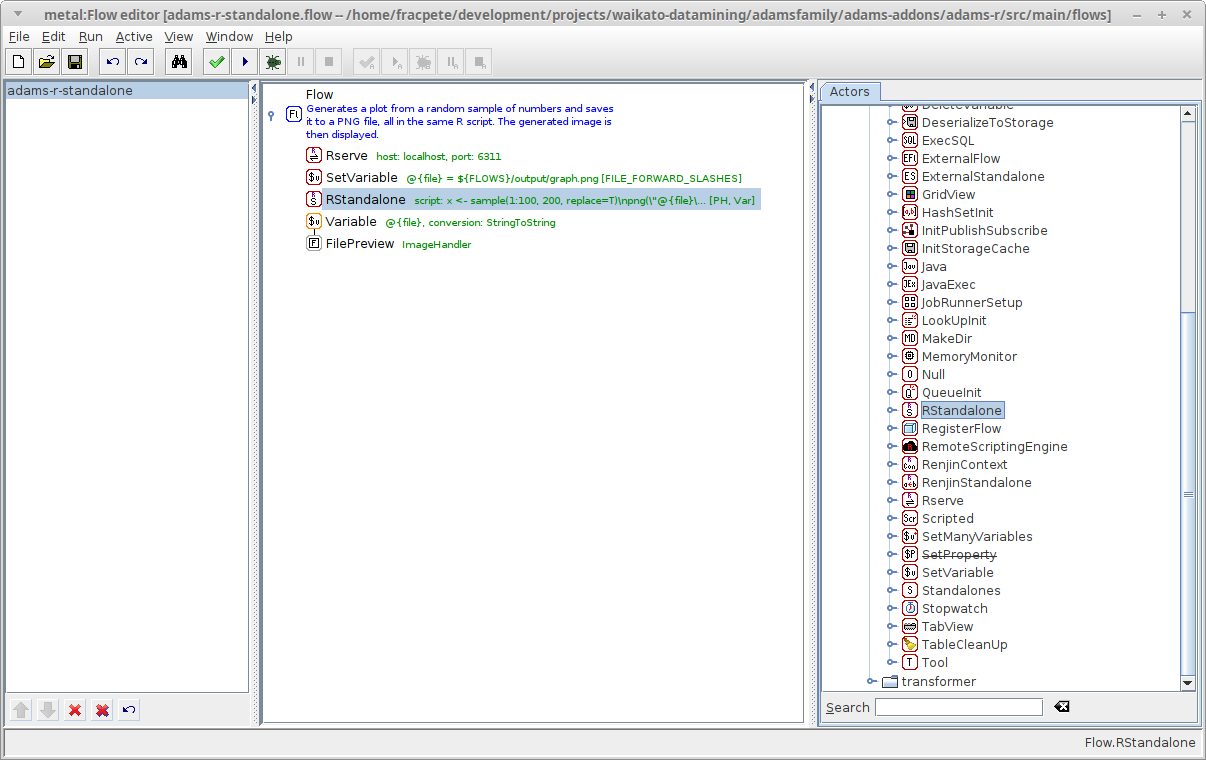
\includegraphics[width=\textwidth]{images/standalone-flow.png}
	\caption{Flow with standalone R script.}
	\label{standalone-flow}
\end{figure}
\begin{figure}[ht]
	\centering
	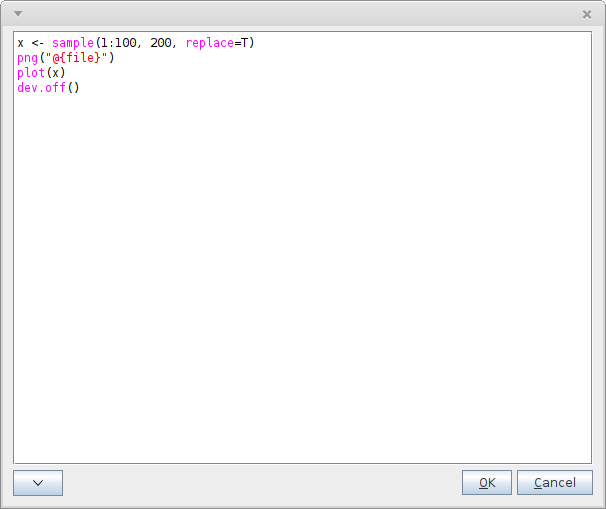
\includegraphics[width=8cm]{images/standalone-script.png}
	\caption{The standalone R script.}
	\label{standalone-script}
\end{figure}
\begin{figure}[ht]
	\centering
	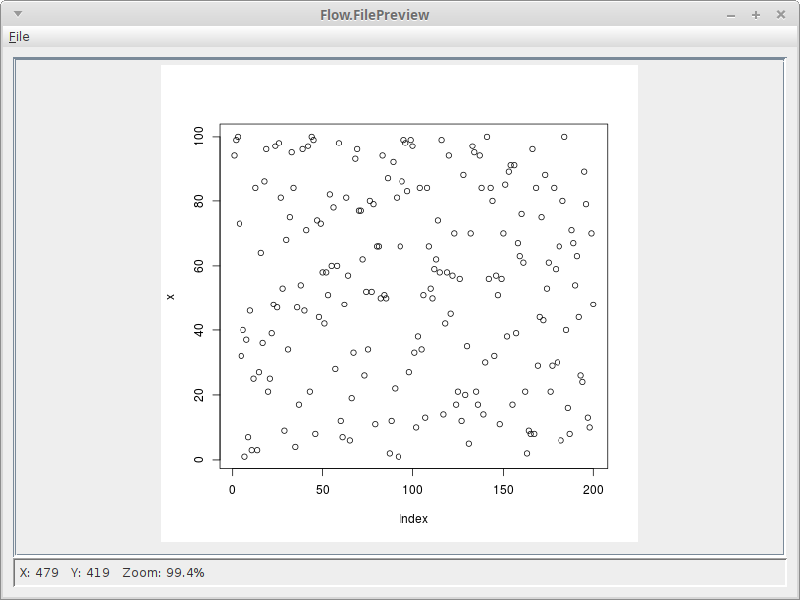
\includegraphics[width=\textwidth]{images/standalone-output.png}
	\caption{The generated plot.}
	\label{standalone-output}
\end{figure}

\clearpage
\subsection{Generating data}
With the \textit{RSource} actor you can use R to generate data and feed it
into the flow like any other ADAMS source actor. The example 
flow\footnote{adams-r-source.flow} in Figure \ref{source-flow} generates
an array of random numbers, transforms it with $log2$ and then uses ADAMS
to plot the array data (see Figure \ref{source-script}).
\begin{figure}[ht]
	\centering
	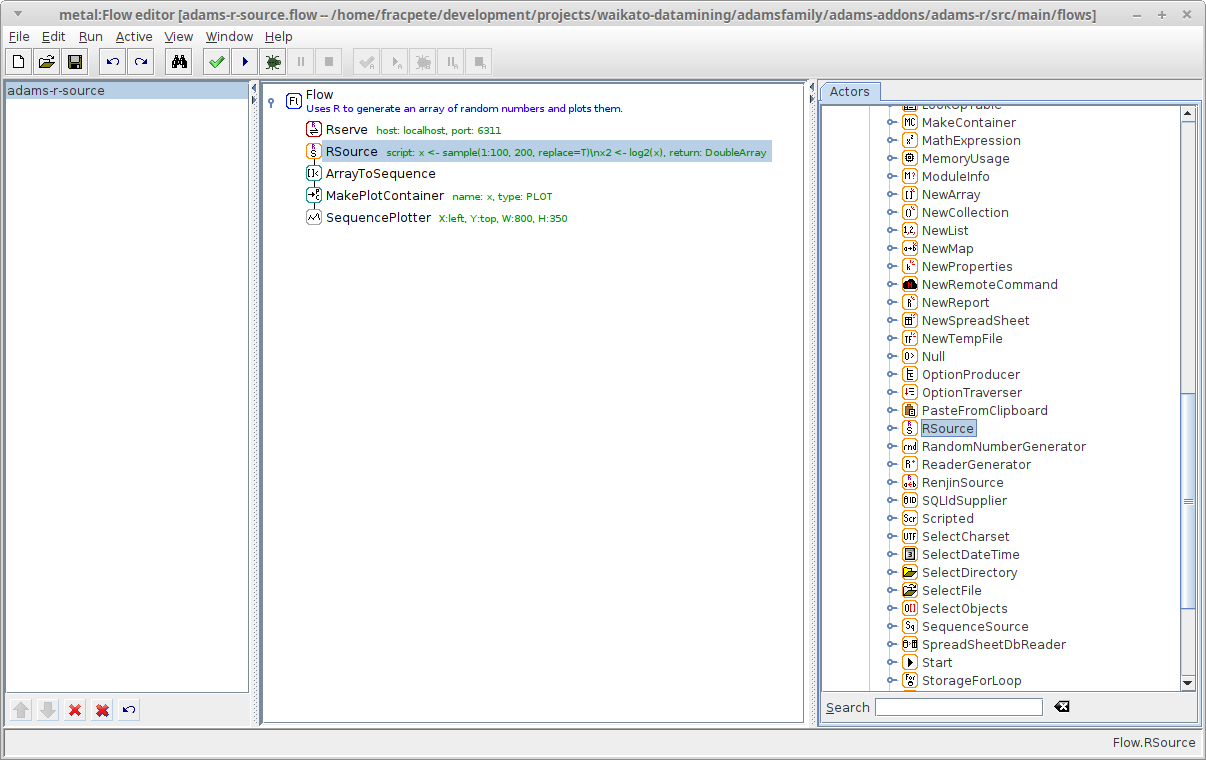
\includegraphics[width=\textwidth]{images/source-flow.png}
	\caption{Flow with RSource actor.}
	\label{source-flow}
\end{figure}
\begin{figure}[ht]
	\centering
	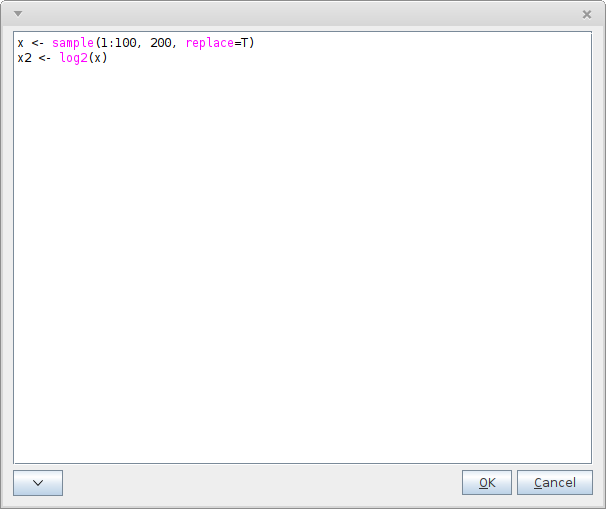
\includegraphics[width=8cm]{images/source-script.png}
	\caption{The data generating R script.}
	\label{source-script}
\end{figure}
\begin{figure}[ht]
	\centering
	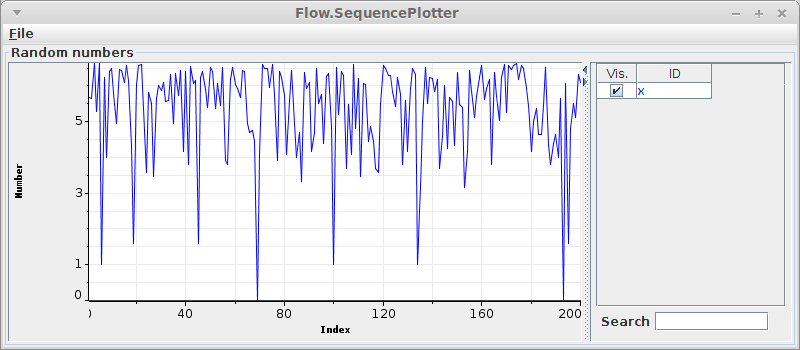
\includegraphics[width=\textwidth]{images/source-output.png}
	\caption{Plot of the random data generated by R.}
	\label{source-output}
\end{figure}

\clearpage
\subsection{Transforming data}
Using the \textit{RTransformer} actor, you can use R to easily transform
data within a flow using R scripts. This allows you to use a plethora
of R packages, all within the workflow environment.

\subsubsection{Double matrix to double}
R offers a lot of transformations and calculation around matrices. The example
flow\footnote{adams-r-matrix\_determinant.flow} turns a CSV string into a
double matrix and calls R to calculate the determinant of the matrix (see
Figure \ref{matrix_determinant-flow}).
\begin{figure}[ht]
	\centering
	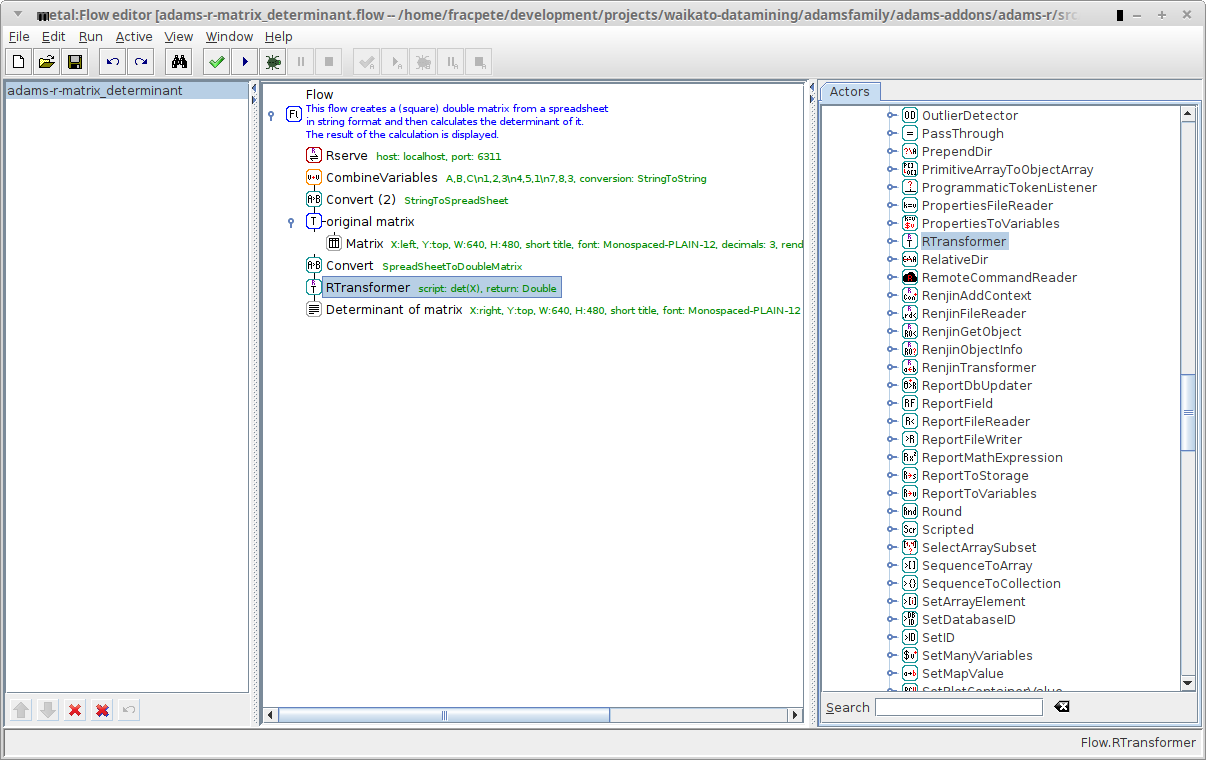
\includegraphics[width=12cm]{images/matrix_determinant-flow.png}
	\caption{Flow for calculating the determinant of a matrix.}
	\label{matrix_determinant-flow}
\end{figure}

\clearpage
\subsubsection{Double matrix to double matrix}
You can also turn matrices into matrices again, rather than just calculating a 
single value as in the previous example. The example
flow\footnote{adams-r-matrix\_transformation.flow} transforms the cells
of the double matrix using $log2$. See Figure \ref{matrix_transformation-flow}.
\begin{figure}[ht]
	\centering
	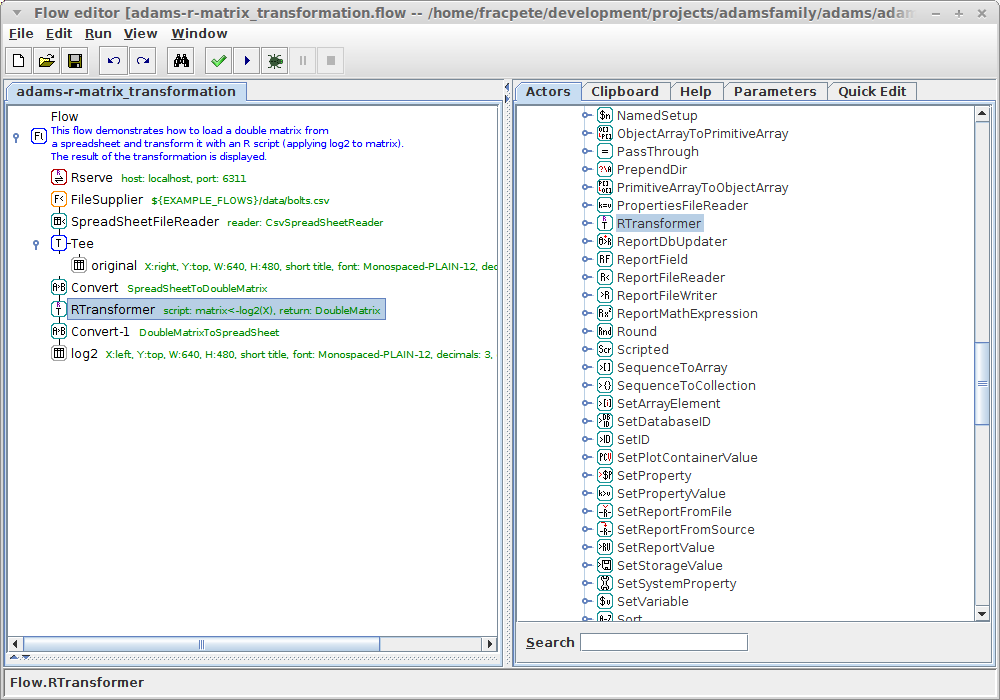
\includegraphics[width=12cm]{images/matrix_transformation-flow.png}
	\caption{Flow for transforming a double matrix.}
	\label{matrix_transformation-flow}
\end{figure}

\clearpage
\subsubsection{Double to double array}
This is an example of a flow that creates a pair of spirals\footnote{adams-r-spirals.flow}.
It makes use of the RTransformer actor along with the Rserve actor to create an
R server. The RTransformer makes use of a given x value and returns a pair of
points, in the form of a double array, that represent the x and y values of the
spiral. See Figures \ref{spirals-flow}, \ref{spirals-rscript} and \ref{spirals-output}.
\begin{figure}[ht]
	\centering
	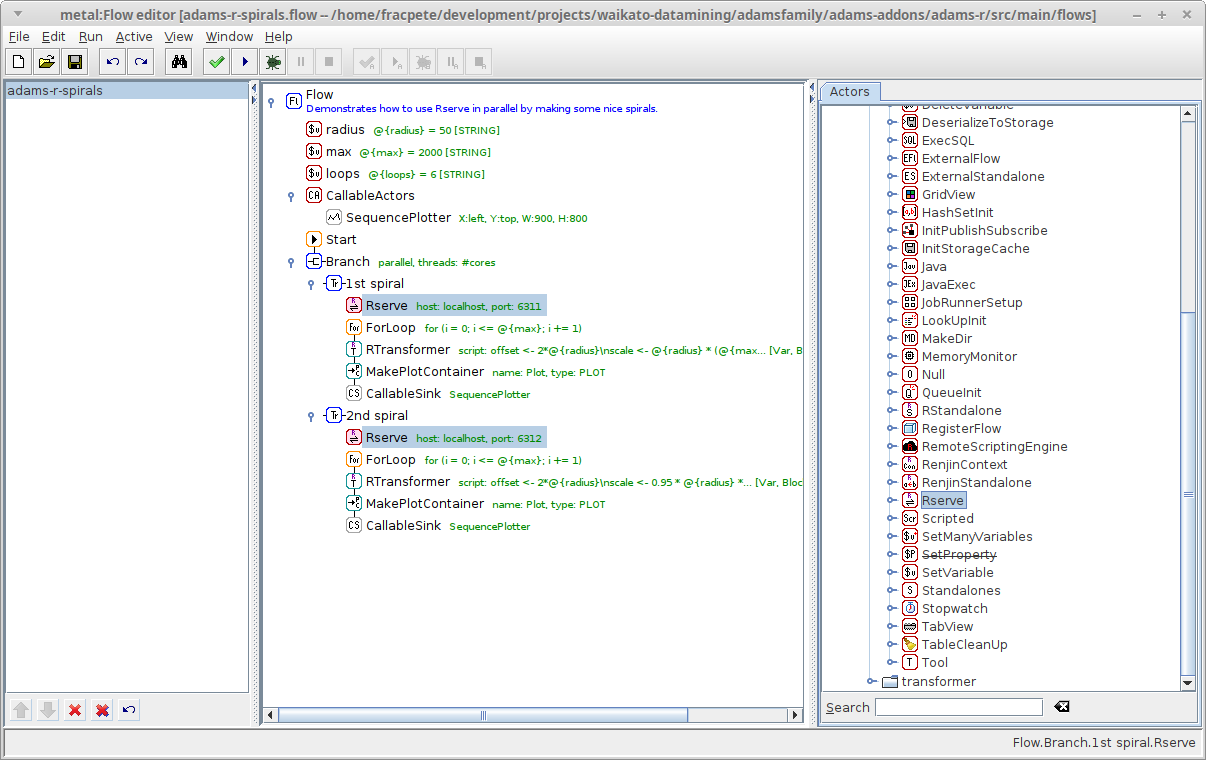
\includegraphics[width=\textwidth]{images/spirals-flow.png}
	\caption{Flow for generating spirals.}
	\label{spirals-flow}
\end{figure}
\begin{figure}[ht]
	\centering
	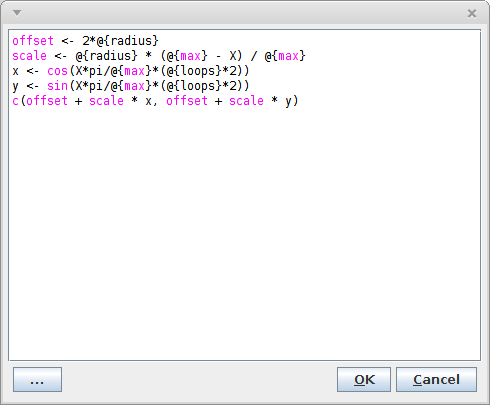
\includegraphics[width=8cm]{images/spirals-rscript.png}
	\caption{The R script for generating the spiral from the RTransformer actor.}
	\label{spirals-rscript}
\end{figure}
\begin{figure}[ht]
	\centering
	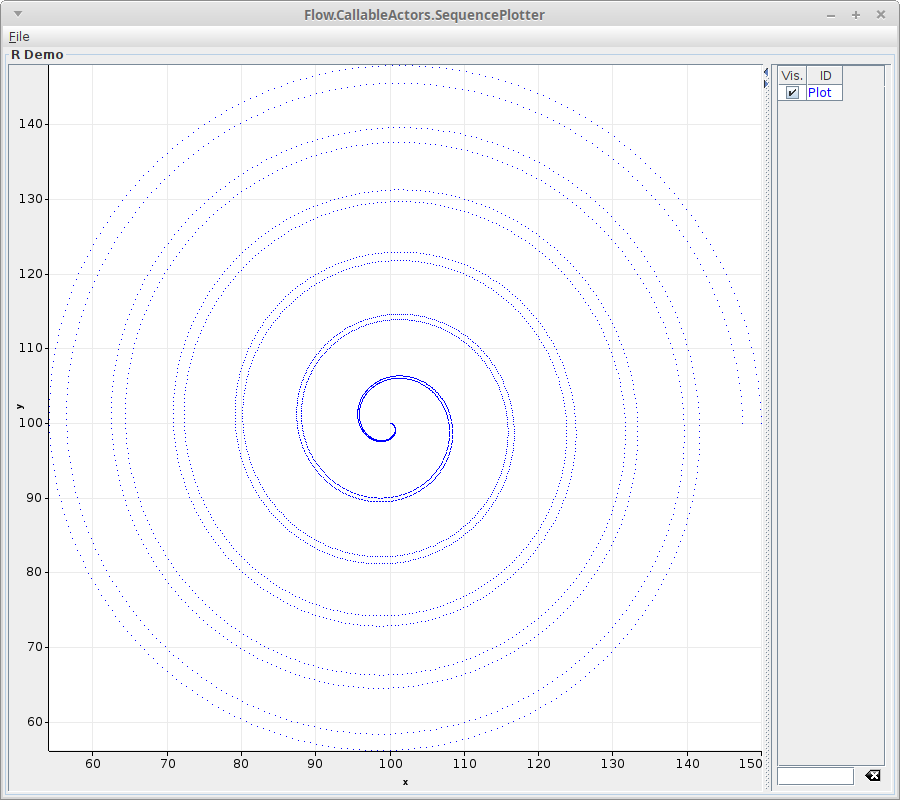
\includegraphics[width=\textwidth]{images/spirals-output.png}
	\caption{The generated spirals plot.}
	\label{spirals-output}
\end{figure}

\clearpage
\subsubsection{Spreadsheet to dataframe}
Dataframes in R can be used to represent tables (or even nested structures).
The example flow\footnote{adams-r-dataframe.flow} loads a spreadsheet and
generates a linear model using the \texttt{lm} command. The resulting 
dataframe is displayed as a spreadsheet again (see Figure \ref{dataframe-flow}).
\begin{figure}[ht]
	\centering
	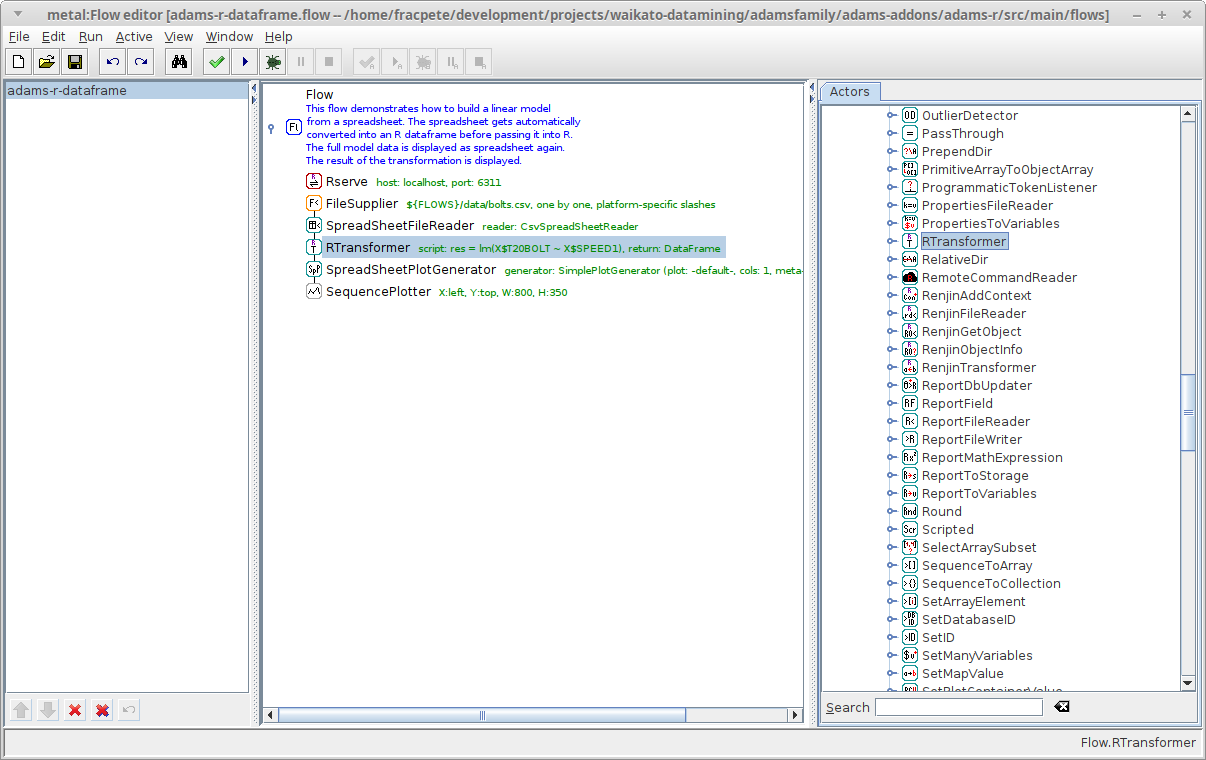
\includegraphics[width=\textwidth]{images/dataframe-flow.png}
	\caption{Flow for generating a linear model from a spreadsheet.}
	\label{dataframe-flow}
\end{figure}
When generating a dataframe as output, you can limit the columns that should
get returned in the spreadsheet. The example flow\footnote{adams-r-dataframe\_columns.flow}
in Figure \ref{dataframe-columns-flow} only retrieves the residuals from the
linear model, which are displayed in Figure \ref{dataframe-columns-output}.
\begin{figure}[ht]
	\centering
	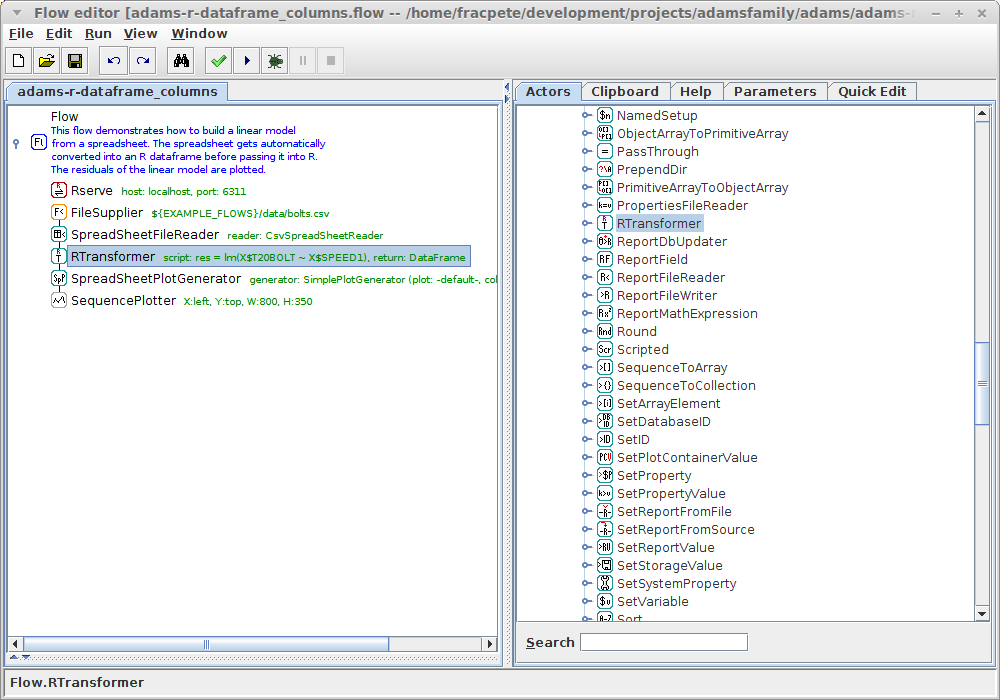
\includegraphics[width=\textwidth]{images/dataframe-columns-flow.png}
	\caption{Flow for plotting the residuals of a linear model.}
	\label{dataframe-columns-flow}
\end{figure}
\begin{figure}[ht]
	\centering
	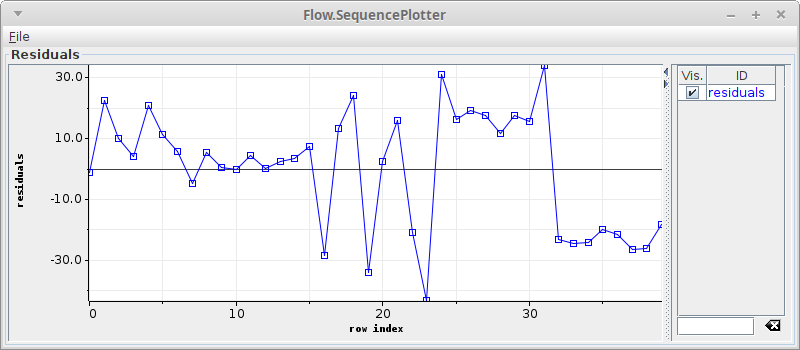
\includegraphics[width=\textwidth]{images/dataframe-columns-output.png}
	\caption{The residuals of a linear model.}
	\label{dataframe-columns-output}
\end{figure}

\clearpage
\subsection{Consuming data}
Using the \textit{RSink} actor, you can \textit{consume} data generated with
ADAMS with an R script. The example flow\footnote{adams-r-sink.flow} in
Figure \ref{sink-flow} shows how to process an array of random doubles 
generated with ADAMS and generating a plot using R. Figure \ref{sink-script}
shows the script used for the plot generation.
\begin{figure}[ht]
	\centering
	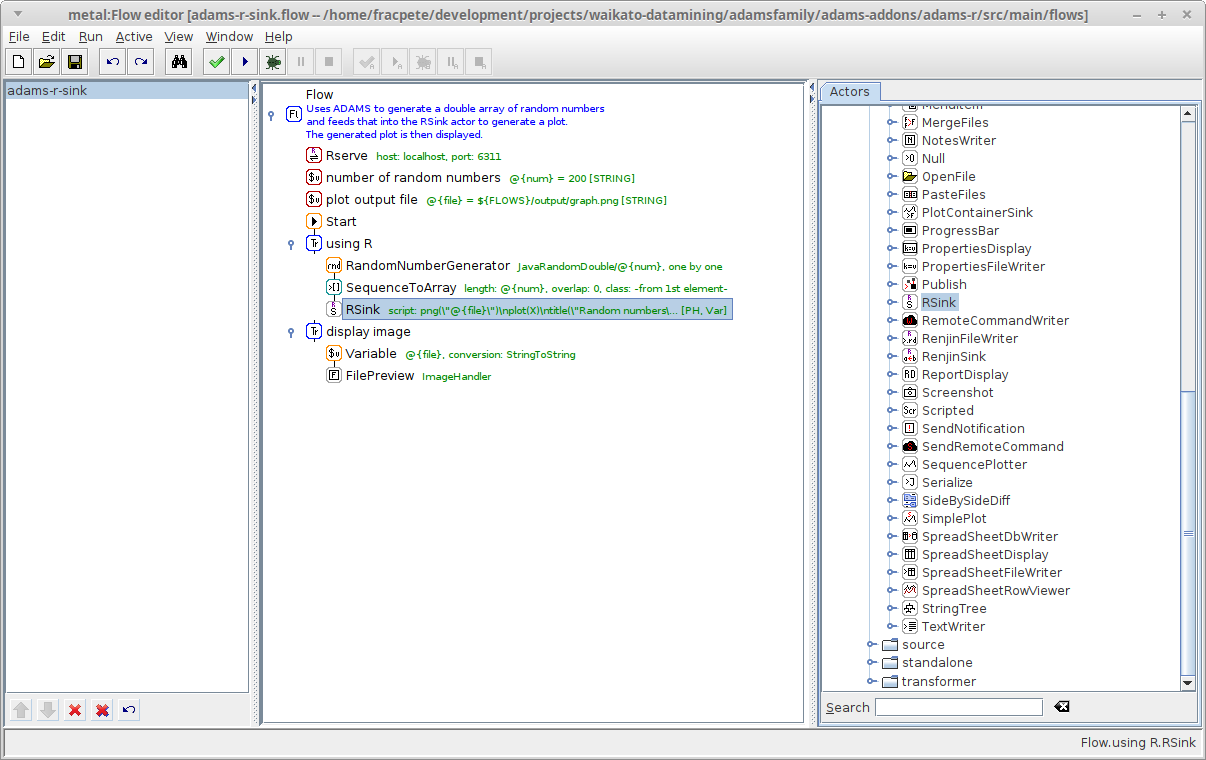
\includegraphics[width=\textwidth]{images/sink-flow.png}
	\caption{Flow with R script acting as sink.}
	\label{sink-flow}
\end{figure}
\begin{figure}[ht]
	\centering
	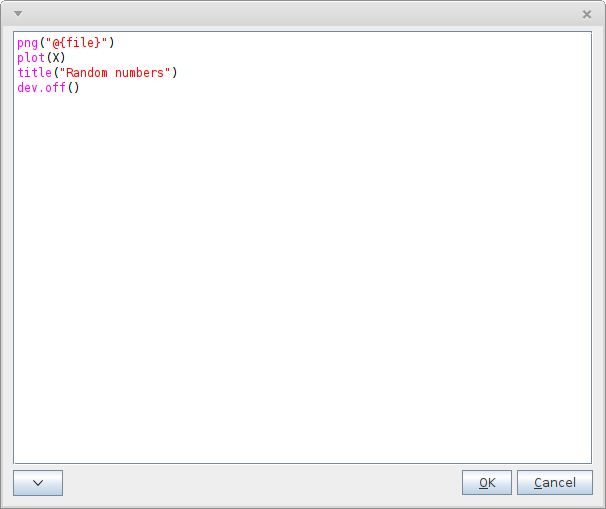
\includegraphics[width=8cm]{images/sink-script.png}
	\caption{The receiving R script.}
	\label{sink-script}
\end{figure}
\begin{figure}[ht]
	\centering
	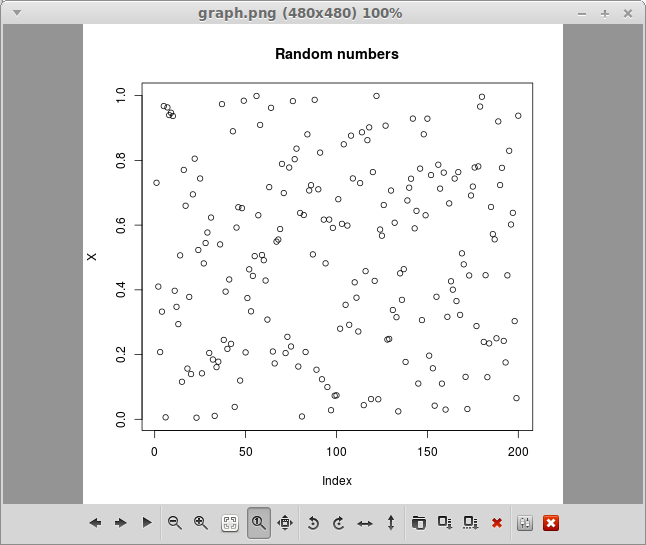
\includegraphics[width=\textwidth]{images/sink-output.png}
	\caption{The plot generated with R.}
	\label{sink-output}
\end{figure}

%%%%%%%%%%%%%%%%%%%%%%%%%%%%%%%%%%%
\chapter{Troubleshooting}
\section{Windows}
\textit{The flow hangs on execution} -- make sure that you only connect 
with one R actor to an Rserve server running on Windows (Linux/Unix/Mac 
allow an arbitrary number of connections). You can place 
\textit{Rserve} standalone actors also inside \textit{Trigger} control 
actors, specifying different ports.\footnote{adams-r-spirals.flow}

\section{Tests}
Junit tests of the flow actors can be disabled using the following command-line 
property:
\begin{verbatim}
-Dadams.test.flow.r.disabled=true
\end{verbatim}
For instance, installing the \textit{adams-r} module without running the R 
flow tests can be achieved with this command-line:
\begin{verbatim}
mvn clean install -Dadams.test.flow.r.disabled=true
\end{verbatim}

%%%%%%%%%%%%%%%%%%%%%%%%%%%%%%%%%%%
% Copyright (c) 2009-2012 by the University of Waikato, Hamilton, NZ. 
% This work is made available under the terms of the 
% Creative Commons Attribution-ShareAlike 4.0 license,
% http://creativecommons.org/licenses/by-sa/4.0/.
%
% Version: $Revision$

\begin{thebibliography}{999}
	% to make the bibliography appear in the TOC
	\addcontentsline{toc}{chapter}{Bibliography}

    % references
	\bibitem{adams}
		\textit{ADAMS} -- Advanced Data mining and Machine learning System \\
		\url{https://adams.cms.waikato.ac.nz/}{}
		
	\bibitem{heatmap}
		\textit{Heat map} -- WikiPedia article \\
		\url{http://en.wikipedia.org/wiki/Heat_map}{}

\end{thebibliography}


\end{document}
